%+++++++++++++++++++++++++++++++++++++++++++++++++++++++++++++++++++++++++++++++
%+++++++++++++++++++++++++++++++++++++++++++++++++++++++++++++++++++++++++++++++
\mysection{Tutorial}
%
This section will show:
\bi
  \item A basic tutorial for a 1D mass and spring-damper with initial displacements, shortest possible model with practically no special settings
  \item A more advanced rigid-body model, including 3D rigid bodies and revolute joints
  \item Links to examples section
\ei
%
A large number of examples, some of them quite advanced, can be found in:
\bi
  \item[] \texttt{main/pythonDev/Examples}
  \item[] \texttt{main/pythonDev/TestModels}
\ei

%+++++++++++++++++++++++++++++++++++++++++++++++++++++++++++++++++++++++++++++++
%+++++++++++++++++++++++++++++++++++++++++++++++++++++++++++++++++++++++++++++++
\mysubsection{Mass-Spring-Damper tutorial}
The Python source code of the first tutorial can be found in the file:
\bi
  \item[] \texttt{main/pythonDev/Examples/springDamperTutorial.py}
\ei
A similar version based on a simplified approach (using a 3D mass point) is available as
\bi
  \item[] \texttt{main/pythonDev/Examples/springDamperTutorialNew.py}
\ei
This tutorial will set up a mass point and a spring damper, dynamically compute the solution and evaluate the reference solution.
\vspace{6pt}\\
We import the exudyn library and the interface for all nodes, objects, markers, loads and sensors:
\pythonstyle\begin{lstlisting}
  import exudyn as exu
  from exudyn.utilities import * #includes itemInterface, graphicsDataUtilities, rigidBodyUtilities, ...
  import numpy as np #not required in general, but convenient for linear algebra
\end{lstlisting}
%
Next, we need a \texttt{SystemContainer}, which contains all computable systems and add a new MainSystem \texttt{mbs}.
Per default, you always should name your system 'mbs' (multibody system), in order to copy/paste code parts from other examples, tutorials and other projects:
\pythonstyle\begin{lstlisting}
  SC = exu.SystemContainer()
  mbs = SC.AddSystem()
\end{lstlisting}
%
In order to check, which version you are using, you can printout the current \codeName\ version. 
The version shown is in line with the issue tracker and marks the number of open/closed issues added to \codeName\ .
Adding \texttt{True} as argument will also print platform-specific information, which is helpful 
in case of reporting some compatibility issues:
\pythonstyle\begin{lstlisting}
  print('EXUDYN version='+exu.GetVersionString(True))
\end{lstlisting}
%
Using the powerful Python language, we can define some variables for our problem, which will also be used for the analytical solution:
\pythonstyle\begin{lstlisting}
  L=0.5               #reference position of mass
  mass = 1.6          #mass in kg
  spring = 4000       #stiffness of spring-damper in N/m
  damper = 8          #damping constant in N/(m/s)
  f =80               #force on mass
\end{lstlisting}
%
For the simple spring-mass-damper system, we need initial displacements and velocities:
\pythonstyle\begin{lstlisting}
  u0=-0.08            #initial displacement
  v0=1                #initial velocity
  x0=f/spring         #static displacement
  print('resonance frequency = '+str(np.sqrt(spring/mass)))
  print('static displacement = '+str(x0))
\end{lstlisting}
%
We first need to add nodes, which provide the coordinates (and the degrees of freedom) to the system.
The following line adds a 3D node for 3D mass point\footnote{Note: Point is an abbreviation for NodePoint, defined in \texttt{itemInterface.py}.}:
\pythonstyle\begin{lstlisting}
  n1=mbs.AddNode(Point(referenceCoordinates = [L,0,0], 
                       initialCoordinates = [u0,0,0], 
                       initialVelocities = [v0,0,0]))
\end{lstlisting}
Here, \texttt{Point} (=\texttt{NodePoint}) is a Python class, which takes a number of arguments defined in the reference manual. The arguments here are \texttt{referenceCoordinates}, which are the coordinates for which the system is defined. The initial configuration is given by \texttt{referenceCoordinates + initialCoordinates}, while the initial state additionally gets \texttt{initialVelocities}.
The command \texttt{mbs.AddNode(...)} returns a \texttt{NodeIndex n1}, which basically contains an integer, which can only be used as node number. This node number will be used lateron to use the node in the object or in the marker.

%
While \texttt{Point} adds 3 unknown coordinates to the system, which need to be solved, we also can add ground nodes, which can be used similar to nodes, but they do not have unknown coordinates -- and therefore also have no initial displacements or velocities. The advantage of ground nodes (and ground bodies) is that no constraints are needed to fix these nodes.
%
Such a ground node is added via:
\pythonstyle\begin{lstlisting}
  nGround=mbs.AddNode(NodePointGround(referenceCoordinates = [0,0,0]))
\end{lstlisting}
%
In the next step, we add an object\footnote{For the moment, we just need to know that objects either depend on one or more nodes, which are usually bodies and finite elements, or they can be connectors, which connect (the coordinates of) objects via markers, see \refSection{sec:overview:modulestructure}.}, which provides equations for coordinates. The \texttt{MassPoint} needs at least a mass (kg) and a node number to which the mass point is attached. Additionally, graphical objects could be attached:
\pythonstyle\begin{lstlisting}
  massPoint = mbs.AddObject(MassPoint(physicsMass = mass, nodeNumber = n1))
\end{lstlisting}
Note that instead of adding a \texttt{NodePoint} and a \texttt{MassPoint} with \texttt{mbs.AddNode(...)}
and \texttt{mbs.AddObject(...)}, there is also a convenient function \texttt{mbs.CreateMassPoint(...)}, which can do everything at once including the option to add gravity.

In order to apply constraints and loads, we need markers. These markers are used as local positions (and frames), where we can attach a constraint lateron. In this example, we work on the coordinate level, both for forces as well as for constraints.
Markers are attached to the according ground and regular node number, additionally using a coordinate number (0 ... first coordinate):
\pythonstyle\begin{lstlisting}
  groundMarker=mbs.AddMarker(MarkerNodeCoordinate(nodeNumber= nGround, 
                                                  coordinate = 0))
  #marker for springDamper for first (x-)coordinate:
  nodeMarker = mbs.AddMarker(MarkerNodeCoordinate(nodeNumber= n1, 
                                                  coordinate = 0))
\end{lstlisting}
This means that constraints are be applied to the first coordinate of node \texttt{n1} via marker with number \texttt{nodeMarker}, which is in fact of type \texttt{MarkerNodeCoordinate}.

Now we add a spring-damper to the markers with numbers \texttt{groundMarker} and the \texttt{nodeMarker}, providing stiffness and damping parameters:
\pythonstyle\begin{lstlisting}
  nC = mbs.AddObject(CoordinateSpringDamper(markerNumbers = [groundMarker, nodeMarker], 
                                       stiffness = spring, 
                                       damping = damper)) 
\end{lstlisting}
%
A load is added to marker \texttt{nodeMarker}, with a scalar load with value \texttt{f}:
\pythonstyle\begin{lstlisting}
  nLoad = mbs.AddLoad(LoadCoordinate(markerNumber = nodeMarker, 
                                     load = f))
\end{lstlisting}
Again, instead of adding a \texttt{MarkerNodeCoordinate} and a \texttt{LoadCoordinate} with \texttt{mbs.AddLoad(...)},
we could just use \texttt{mbs.CreateForce(...)} to add a 3D force vector.
For specific joints, there are also \texttt{mbs.Create...(...)} functions.

Finally, a sensor is added to the coordinate constraint object with number \texttt{nC}, requesting the \texttt{outputVariableType} \texttt{Force}:
\pythonstyle\begin{lstlisting}
  mbs.AddSensor(SensorObject(objectNumber=nC, fileName='groundForce.txt', 
                             outputVariableType=exu.OutputVariableType.Force))
\end{lstlisting}
Note that sensors can be attached, e.g., to nodes, bodies, objects (constraints) or loads.
%
As our system is fully set, we can print the overall information and assemble the system to make it ready for simulation:
\pythonstyle\begin{lstlisting}
  print(mbs)     #show system properties
  mbs.Assemble() #prepare for simulation
\end{lstlisting}
%
We will use time integration and therefore define a number of steps (fixed step size; must be provided) and the total time span for the simulation:
\pythonstyle\begin{lstlisting}
  tEnd = 1     #end time of simulation
  h = 0.001    #step size; leads to 1000 steps
\end{lstlisting}
%
All settings for simulation, see according reference section, can be provided in a structure given from \texttt{exu.SimulationSettings()}. Note that this structure will contain all default values, and only non-default values need to be provided:
\pythonstyle\begin{lstlisting}
  simulationSettings = exu.SimulationSettings()
  simulationSettings.solutionSettings.solutionWritePeriod = 5e-3 #output interval general
  simulationSettings.solutionSettings.sensorsWritePeriod = 5e-3  #output interval of sensors
  simulationSettings.timeIntegration.numberOfSteps = int(tEnd/h) #must be integer
  simulationSettings.timeIntegration.endTime = tEnd
  simulationSettings.displayComputationTime = True               #show how fast
\end{lstlisting}
%
In order to see some solver output, we must set \texttt{verboseMode} to 1 (higher values gives detailed output per step).
Furthermore, we can show information on computation time (which may cost some overhead in computation!):
\pythonstyle\begin{lstlisting}
  simulationSettings.timeIntegration.verboseMode = 1             #show some solver output
  simulationSettings.displayComputationTime = True               #show how fast
\end{lstlisting}
We are using a generalized alpha solver, where numerical damping is needed for index 3 constraints. As we have only spring-dampers, we can set the spectral radius to 1, meaning no numerical damping:
\pythonstyle\begin{lstlisting}
  simulationSettings.timeIntegration.generalizedAlpha.spectralRadius = 1
\end{lstlisting}
%
In order to visualize the results online, a renderer can be started. As our computation will be very fast, it is a good idea to wait for the user to press SPACE, before starting the simulation (uncomment second line):
\pythonstyle\begin{lstlisting}
  exu.StartRenderer()              #start graphics visualization
  #mbs.WaitForUserToContinue()     #wait for SPACE bar or 'Q' to continue (in render window!)
\end{lstlisting}
As the simulation is still very fast, we will not see the motion of our node. Using a very small step size of, e.g., \texttt{h=1e-7} in the lines above allows us to visualize the resulting oscillations in realtime.

%
Finally, we start the solver, by telling which system to be solved, solver type and the simulation settings:
\pythonstyle\begin{lstlisting}
  exu.SolveDynamic(mbs, simulationSettings)
\end{lstlisting}
%

After simulation, our renderer needs to be stopped (otherwise it will stop unsafely as soon as the Python kernel is stopped or restarted). 
Sometimes you would like to wait until closing the render window, using \texttt{WaitForRenderEngineStopFlag()}:
\pythonstyle\begin{lstlisting}
  #SC.WaitForRenderEngineStopFlag()#wait for pressing 'Q' to quit
  exu.StopRenderer()               #safely close rendering window!
\end{lstlisting}
%
If you run this code, e.g. in Spyder or Visual Studio Code, it may take a 1-2 seconds to complete. However, the time spent is only related to some overhead in the Python environment and for the visualization. The simulation itself will only take around 3-10 milliseconds, in which a large overhead is due to file writing.

There are several ways to evaluate results, see the reference pages. In the following we take the final value of node \texttt{n1} and read its 3D position vector:
\pythonstyle\begin{lstlisting}
  #evaluate final (=current) output values
  u = mbs.GetNodeOutput(n1, exu.OutputVariableType.Position)
  print('displacement=',u)
\end{lstlisting}
%
The following code generates a reference (exact) solution for our example:
\pythonstyle\begin{lstlisting}
  import matplotlib.pyplot as plt
  import matplotlib.ticker as ticker

  omega0 = np.sqrt(spring/mass)          #eigen frequency of undamped system
  dRel = damper/(2*np.sqrt(spring*mass)) #dimensionless damping
  omega = omega0*np.sqrt(1-dRel**2)      #eigen freq of damped system
  C1 = u0-x0 #static solution needs to be considered!
  C2 = (v0+omega0*dRel*C1) / omega       #C1, C2 are coeffs for solution
  steps = int(tEnd/h)                    #use same steps for reference solution

  refSol = np.zeros((steps+1,2))
  for i in range(0,steps+1):
    t = tEnd*i/steps
    refSol[i,0] = t
    refSol[i,1] = np.exp(-omega0*dRel*t)*(C1*np.cos(omega*t)+C2*np.sin(omega*t))+x0

  plt.plot(refSol[:,0], refSol[:,1], 'r-', label='displacement (m); exact solution')
\end{lstlisting}
%
Now we can load our results from the default solution file \texttt{coordinatesSolution.txt}, which is in the same
directory as your Python tutorial file. 
\mybold{Note} that the visualization of results can be simplified considerably using the \texttt{PlotSensor(...)} utility function as shown in the \mybold{Rigid body and joints tutorial}!

For reading the file containing commented lines (this does not work in binary mode!), we use a numpy feature and finally plot the displacement of coordinate 0 or our mass point\footnote{\texttt{data[:,0]} contains the simulation time, \texttt{data[:,1]} contains displacement of (global) coordinate 0, \texttt{data[:,2]} contains displacement of (global) coordinate 1, ...)}:
\pythonstyle\begin{lstlisting}
  data = np.loadtxt('coordinatesSolution.txt', comments='#', delimiter=',')
  plt.plot(data[:,0], data[:,1], 'b-', label='displacement (m); numerical solution') 
\end{lstlisting}
The sensor result can be loaded in the same way. The sensor output format contains time in the first column and sensor values in the remaining columns. The number of columns depends on the 
sensor and the output quantity (scalar, vector, ...):
\pythonstyle\begin{lstlisting}
  data = np.loadtxt('groundForce.txt', comments='#', delimiter=',')
  plt.plot(data[:,0], data[:,1]*1e-3, 'g-', label='force (kN)')
\end{lstlisting}
%
In order to get a nice plot within Spyder, the following options can be used\footnote{note, in some environments you need finally the command \texttt{plt.show()}}:
\pythonstyle\begin{lstlisting}
  ax=plt.gca() # get current axes
  ax.grid(True, 'major', 'both')
  ax.xaxis.set_major_locator(ticker.MaxNLocator(10))
  ax.yaxis.set_major_locator(ticker.MaxNLocator(10))
  plt.legend() #show labels as legend
  plt.tight_layout()
  plt.show() 
\end{lstlisting}
%
The matplotlib output should look as shown in \fig{fig_tutorial_springDamper}.
%
\LatexRSTfigure{figures/plotSpringDamper}{fig_tutorial_springDamper}{12cm}{400}{Output of spring-damper tutorial.}
%
%
%\ignoreRST{\begin{center}
  %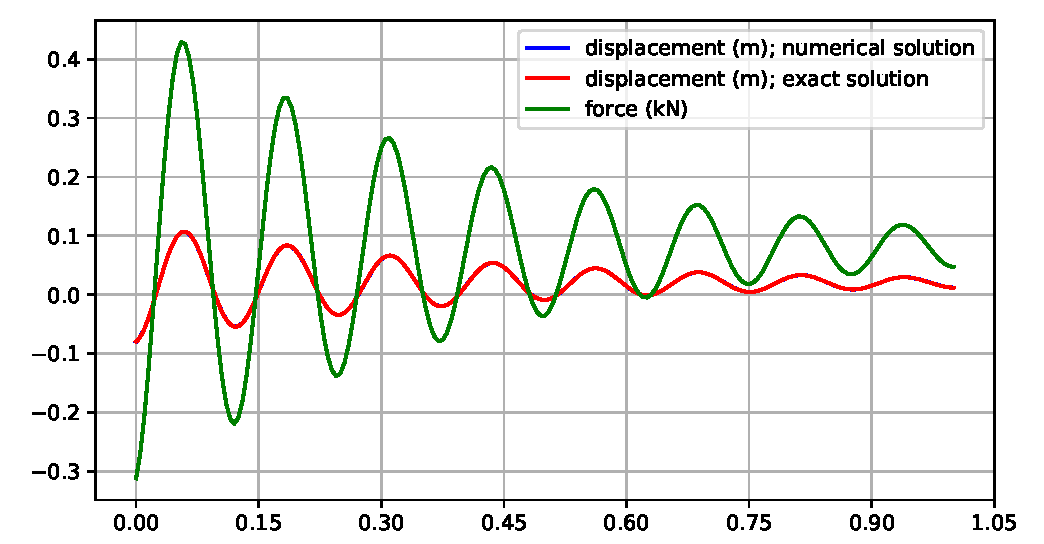
\includegraphics[height=6cm]{../demo/screenshots/plotSpringDamper}
%\end{center}}
%\onlyRST{
%
%.. image:: docs/theDoc/figures/plotSpringDamper.png
   %:width: 400
%
%}



%++++++++++++++++++++++++++++++++++++++++++++++++++++++++++++++++++++++++++++++++++++++++++++++++++++++++++++++
%++++++++++++++++++++++++++++++++++++++++++++++++++++++++++++++++++++++++++++++++++++++++++++++++++++++++++++++
%++++++++++++++++++++++++++++++++++++++++++++++++++++++++++++++++++++++++++++++++++++++++++++++++++++++++++++++
\newpage
\mysubsectionlabel{Rigid body and joints tutorial}{sec:tutorial:rigidBodyJoints}
The Python source code of the first tutorial, based on the simple description of revolute joints, can be found in the file:
\bi
  \item[] \texttt{main/pythonDev/Examples/rigidBodyTutorial3.py}
\ei
For alternative approaches, see
\bi
  \item[] \texttt{main/pythonDev/Examples/rigidBodyTutorial3withMarkers.py}
  \item[] \texttt{main/pythonDev/Examples/rigidBodyTutorial2.py}
\ei
This tutorial will set up a multibody system containing a ground, two rigid bodies and two revolute joints driven by gravity, compare a 3D view of the example in \fig{fig_RigidBodyTutorialView}.
%
\LatexRSTfigure{figures/TutorialRigidBody1desc}{fig_RigidBodyTutorialView}{14cm}{400}{Render view of rigid body tutorial, showing objects, nodes (N0, N1), and loads.}
%
%\ignoreRST{\fig{fig_RigidBodyTutorialView}.} \onlyRST{the figure above.}
%\ignoreRST{\begin{figure}[tbph]
  %\begin{center}
    %\includegraphics[width=0.9\textwidth]{figures/TutorialRigidBody1desc}
  %\end{center}
  %\caption{Render view of rigid body tutorial, showing objects, nodes (N0, N1), and loads.}
  %\label{fig_RigidBodyTutorialView}
%\end{figure}}
%\onlyRST{
%
%.. image:: docs/theDoc/figures/TutorialRigidBody1desc.png
%   :width: 400
%
%}
\horizontalRuler\\
\noindent We first import the exudyn library and the interface for all nodes, objects, markers, loads and sensors:
\pythonstyle\begin{lstlisting}
  import exudyn as exu
  from exudyn.utilities import * #includes itemInterface, graphicsDataUtilities and rigidBodyUtilities
  import numpy as np #for postprocessing
\end{lstlisting}
The submodule \texttt{exudyn.utilities} contains helper functions for graphics representation, 3D rigid bodies and joints.

\noindent As in the first tutorial, we need a \texttt{SystemContainer} and add a new MainSystem \texttt{mbs}:
\pythonstyle\begin{lstlisting}
  SC = exu.SystemContainer()
  mbs = SC.AddSystem()
\end{lstlisting}

\noindent We define some geometrical parameters for lateron use.
\pythonstyle\begin{lstlisting}
  #physical parameters
  g =     [0,-9.81,0] #gravity
  L = 1               #length
  w = 0.1             #width
  bodyDim=[L,w,w]     #body dimensions
  p0 =    [0,0,0]     #origin of pendulum
  pMid0 = np.array([L*0.5,0,0]) #center of mass, body0
\end{lstlisting}

\noindent We add an empty ground body, using default values. It's origin is at [0,0,0] and here we use no visualization.
\pythonstyle\begin{lstlisting}
  #ground body, located at specific position (there could be several ground objects)
  oGround = mbs.CreateGround(referencePosition=[0,0,0])
\end{lstlisting}
%oGround = mbs.AddObject(ObjectGround())

\horizontalRuler\\
\noindent For physical parameters of the rigid body, we can use the class \texttt{RigidBodyInertia}, which allows to define mass, center of mass (COM) and inertia parameters, as well as shifting COM or adding inertias.
The \texttt{RigidBodyInertia} can be used directly to create rigid bodies. Special derived classes can be use to define rigid body inertias for cylinders, cubes, etc., so we use a cube here:
\pythonstyle\begin{lstlisting}
  #first link:
  #inertia for cubic body with dimensions in sideLengths
  iCube0 = InertiaCuboid(density=5000, sideLengths=bodyDim)
  iCube0 = iCube0.Translated([-0.25*L,0,0]) #transform COM, COM not at reference point!
\end{lstlisting}
Note that the COM is translated in axial direction, while it would be at the body's local position [0,0,0] by default!

\noindent For visualization, we add some graphics for the body defined as a 3D cube with center point and dimensions; additionally we draw a basis (three RGB-vectors) at the COM:
\pythonstyle\begin{lstlisting}
  #graphics for body
  graphicsBody0 = GraphicsDataOrthoCubePoint(centerPoint=[0,0,0],size=[L,w,w],color=color4red)
  graphicsCOM0 = GraphicsDataBasis(origin=iCube0.com, length=2*w)
\end{lstlisting}

\noindent Now we have defined all data for the link (rigid body). We could use \texttt{mbs.AddNode(NodeRigidBodyEP(...))} and \texttt{mbs.AddObject(ObjectRigidBody(...))} to create a node and a body, but the \texttt{MainSystem} since V1.6.110 offers a much more comfortable function:
\pythonstyle\begin{lstlisting}
  #create node, add body and gravity load:
  b0=mbs.CreateRigidBody(inertia = iCube0, #includes COM
                         referencePosition = pMid0,
                         gravity = g,
                         graphicsDataList = [graphicsCOM0, graphicsBody0])
\end{lstlisting}
which also adds a gravity load and could also set initial velocities, if wanted. Note that much more options are available for this function, e.g.,
we could define a \texttt{nodeType} for the underlying formulation of the rigid body node, see \refSection{sec:NodeType}.
We can use 
\bi
\item \texttt{RotationEulerParameters}: for fast computation, but leads to an additional algebraic equation and thus needs an implicit solver
\item \texttt{RotationRxyz}: contains a singularity if the second angle reaches +/- 90 degrees, but no algebraic equations
\item \texttt{RotationRotationVector}: for usage with Lie group integrators, especially with explicit integration, singularities are bypassed; leads to fewest unknowns and usually less Newton iterations
\ei

\noindent We now add a revolute joint around the (global) z-axis. 
We have several possibilities, which are shown in the following.
For the \mybold{first two possibilities only}, following \texttt{rigidBodyTutorial3withMarkers.py}, we need the following markers
\pythonstyle\begin{lstlisting}
  #markers for ground and rigid body (not needed for option 3):
  markerGround = mbs.AddMarker(MarkerBodyRigid(bodyNumber=oGround, localPosition=[0,0,0]))
  markerBody0J0 = mbs.AddMarker(MarkerBodyRigid(bodyNumber=b0, localPosition=[-0.5*L,0,0]))
\end{lstlisting}

\noindent The very general \mybold{option 1} is to use the \texttt{GenericJoint}, that can be used to define any kind of joint with translations and rotations fixed or free,
\pythonstyle\begin{lstlisting}
  #revolute joint option 1:
  mbs.AddObject(GenericJoint(markerNumbers=[markerGround, markerBody0J0], 
                             constrainedAxes=[1,1,1,1,1,0],
                             visualization=VObjectJointGeneric(axesRadius=0.2*w, 
                                                               axesLength=1.4*w)))
\end{lstlisting}
In addition, transformation matrices (\texttt{rotationMarker0/1}) can be added, see the joint description.

\noindent \mybold{Option 2} is using the revolute joint, which allows a free rotation around the local z-axis of marker 0 (\texttt{markerGround} in our example)
\pythonstyle\begin{lstlisting}
  #revolute joint option 2:
  mbs.AddObject(ObjectJointRevoluteZ(markerNumbers = [markerGround, markerBody0J0], 
                                     rotationMarker0=np.eye(3),
                                     rotationMarker1=np.eye(3),
                                     visualization=VObjectJointRevoluteZ(axisRadius=0.2*w, 
                                                                         axisLength=1.4*w)
                                     )) 
\end{lstlisting}
Additional transformation matrices (\texttt{rotationMarker0/1}) can be added in order to chose any rotation axis.

\noindent Note that an error in the definition of markers for the joints can be also detected in the render window (if you completed the example), e.g., if you change the following marker in the lines above,
\pythonstyle\begin{lstlisting}
  #example if wrong marker position is chosen:
  markerBody0J0 = mbs.AddMarker(MarkerBodyRigid(bodyNumber=b0, localPosition=[-0.4*L,0,0]))
\end{lstlisting}
$\ra$ you will see a misalignment of the two parts of the joint by \texttt{0.1*L}.
The latter approach is very general and will also work for any kind of flexible bodies.

\noindent Due to the fact that the definition of markers for general joints is tedious, \mybold{option 3} is based on a MainSystem function, which allows to attach revolute joints immediately to bodies and defining the rotation axis only once for the joint:
\pythonstyle\begin{lstlisting}
  #revolute joint option 3:
  mbs.CreateRevoluteJoint(bodyNumbers=[oGround, b0], position=[0,0,0], 
                          axis=[0,0,1], axisRadius=0.2*w, axisLength=1.4*w)
\end{lstlisting}
For the latter option, there are more arguments that may be specified, e.g., the axis and position can also be defined in the local frame of the first body.

\horizontalRuler\\
\noindent The second link and the according joint can be set up in a very similar way.
For visualization, we need to add some graphics for the body defined as a RigidLink GraphicsData function:
\pythonstyle\begin{lstlisting}
  #second link, simple graphics:
  graphicsBody1 = GraphicsDataRigidLink(p0=[0,0,-0.5*L],p1=[0,0,0.5*L], 
                                        axis0=[1,0,0], axis1=[0,0,0], radius=[0.06,0.05], 
                                        thickness = 0.1, width = [0.12,0.12], 
                                        color=color4lightgreen)

  b1=mbs.CreateRigidBody(inertia = InertiaCuboid(density=5000, sideLengths=[0.1,0.1,1]),
                         referencePosition = np.array([L,0,0.5*L]), 
                         gravity = g,
                         graphicsDataList = [graphicsBody1])
\end{lstlisting}

\noindent The revolute joint in this case has a free rotation around the global x-axis:
\pythonstyle\begin{lstlisting}
  #revolute joint (free x-axis)
  mbs.CreateRevoluteJoint(bodyNumbers=[b0, b1], position=[L,0,0], 
                          axis=[1,0,0], axisRadius=0.2*w, axisLength=1.4*w)
\end{lstlisting}

\noindent Optionally, we could also add forces or torques onto bodies
\pythonstyle\begin{lstlisting}
  #forces can be added like in the following
  force = [0,0.5,0]       #0.5N   in y-direction
  torque = [0.1,0,0]      #0.1Nm around x-axis
  mbs.CreateForce(bodyNumber=b1,
                  loadVector=force,
                  localPosition=[0,0,0.5], #at tip
                  bodyFixed=False) #if True, direction would corotate with body
  mbs.CreateTorque(bodyNumber=b1, 
                  loadVector=torque,
                  localPosition=[0,0,0],   #at body's reference point/center
                  bodyFixed=False) #if True, direction would corotate with body
\end{lstlisting}

\noindent Finally, we also add a sensor for some output of the double pendulum:
\pythonstyle\begin{lstlisting}
  #position sensor at tip of body1
  sens1=mbs.AddSensor(SensorBody(bodyNumber = b1, localPosition = [0,0,0.5*L],
                                 fileName = 'solution/sensorPos.txt',
                                 outputVariableType = exu.OutputVariableType.Position))
\end{lstlisting}
%

\horizontalRuler\\
\noindent Before simulation, we need to call \texttt{Assemble()} for our system, which links objects, nodes, ..., assigns initial values and does further pre-computations and checks:
\pythonstyle\begin{lstlisting}
  mbs.Assemble()
\end{lstlisting}
After \texttt{Assemble()}, markers, nodes, objects, etc. are linked and we can analyze the internal structure. First, we can print out useful information, either just typing \texttt{mbs} in the iPython console to print out overal information:
\plainlststyle
\begin{lstlisting}
  <systemData: 
    Number of nodes= 2
    Number of objects = 5
    Number of markers = 8
    Number of loads = 4
    Number of sensors = 1
    Number of ODE2 coordinates = 14
    Number of ODE1 coordinates = 0
    Number of AE coordinates   = 12
    Number of data coordinates   = 0
    For details see mbs.systemData, mbs.sys and mbs.variables
  >
\end{lstlisting}
%
Note that there are 2 nodes for the two rigid bodies. The five objects are due to ground object, 2 rigid bodies and 2 revolute joints.
The meaning of markers can be seen in the graphical representation described below.

\noindent Furthermore, we can print the full internal information as a dictionary using:
\pythonstyle\begin{lstlisting}
  mbs.systemData.Info() #show detailed information
\end{lstlisting}
which results in the following output (shortened):
\plainlststyle
\begin{lstlisting}
  node0:
      {'nodeType': 'RigidBodyEP', 'referenceCoordinates': [0.5, 0.0, 0.0, 1.0, 0.0, 0.0, 0.0], 'addConstraintEquation': True, 'initialCoordinates': [0.0, 0.0, 0.0, 0.0, 0.0, 0.0, 0.0], 'initialVelocities': [0.0, 0.0, 0.0, 0.0, 0.0, 0.0, 0.0], 'name': 'node0', 'Vshow': True, 'VdrawSize': -1.0, 'Vcolor': [-1.0, -1.0, -1.0, -1.0]}
  node1:
      {'nodeType': 'RigidBodyEP', 'referenceCoordinates': [1.0, 0.0, 0.5, 1.0, 0.0, 0.0, 0.0], 'addConstraintEquation': True, 'initialCoordinates': [0.0, 0.0, 0.0, 0.0, 0.0, 0.0, 0.0], 'initialVelocities': [0.0, 0.0, 0.0, 0.0, 0.0, 0.0, 0.0], 'name': 'node1', 'Vshow': True, 'VdrawSize': -1.0, 'Vcolor': [-1.0, -1.0, -1.0, -1.0]}
  object0:
      {'objectType': 'Ground', 'referencePosition': [0.0, 0.0, 0.0], 'name': 'object0', 'Vshow': True, 'VgraphicsDataUserFunction': 0, 'Vcolor': [-1.0, -1.0, -1.0, -1.0], 'VgraphicsData': {'TODO': 'Get graphics data to be implemented'}}
  object1:
      {'objectType': 'RigidBody', 'physicsMass': 50.0, 'physicsInertia': [0.08333333333333336, 7.333333333333334, 7.333333333333334, 0.0, 0.0, 0.0], 'physicsCenterOfMass': [-0.25, 0.0, 0.0], 'nodeNumber': 0, 'name': 'object1', 'Vshow': True, 'VgraphicsDataUserFunction': 0, 'VgraphicsData': {'TODO': 'Get graphics data to be implemented'}}
  object2:
      {'objectType': 'JointRevolute', 'markerNumbers': [3, 4], 'rotationMarker0': [[0.0, 1.0, 0.0], [-1.0, 0.0, 0.0], [0.0, 0.0, 1.0]], 'rotationMarker1': [[0.0, 1.0, 0.0], [-1.0, 0.0, 0.0], [0.0, 0.0, 1.0]], 'activeConnector': True, 'name': 'object2', 'Vshow': True, 'VaxisRadius': 0.019999999552965164, 'VaxisLength': 0.14000000059604645, 'Vcolor': [-1.0, -1.0, -1.0, -1.0]}
  object3:
  ...
\end{lstlisting}

\noindent Sometimes it is hard to understand the degree of freedom for the constrained system. Furthermore, we may have added -- by error --
redundant constraints, which are not solvable or at least cause solver problems. Both can be checked with the command:
\pythonstyle\begin{lstlisting}
  mbs.ComputeSystemDegreeOfFreedom(verbose=True) #print out DOF and further information
\end{lstlisting}
This will print:
\begin{lstlisting}
  ODE2 coordinates          = 14
  total constraints         = 12
  redundant constraints     = 0
  pure algebraic constraints= 0
  degree of freedom         = 2
\end{lstlisting}
We see that there are 14 ODE2 coordinates from the two nodes that are based on Euler parameters. The two joints add $2\times 5$ constraints and there are 2 additional Euler parameter constraints, giving a degree of freedom of 2 (as expected ...).

\noindent You can try and duplicate the code for the second revolute joint:
\pythonstyle\begin{lstlisting}
  #add a second constraint for bodies b0 and b1:
  mbs.CreateRevoluteJoint(bodyNumbers=[b0, b1], ...)
\end{lstlisting}
such that we have two identical joints (which would be unwanted, in general). This would give 
\begin{lstlisting}
  ODE2 coordinates          = 14
  total constraints         = 17
  redundant constraints     = 5
  pure algebraic constraints= 0
  degree of freedom         = 2
\end{lstlisting}
which clearly shows the 5 redundant constraints, which will lead to a solver failure (except for the \texttt{EigenDense} solver, see there). In practical cases, redundant constraints may be much more involved, but can be detected in this way.

\noindent A graphical representation of the internal structure of the model can be shown using the command \texttt{DrawSystemGraph}:
\pythonstyle\begin{lstlisting}
  mbs.DrawSystemGraph(useItemTypes=True) #draw nice graph of system
\end{lstlisting}
%For the output see \ignoreRST{\fig{fig_DrawSystemGraphExample}}\onlyRST{the figure below}. 
For the output see \fig{fig_DrawSystemGraphExample}. 
Note that obviously, markers are always needed to connect objects (or nodes) as well as loads. We can also see, that 2 markers MarkerBodyRigid1 and MarkerBodyRigid2 are unused, which is no further problem for the model and also does not require additional computational resources (except for some bytes of memory). Having isolated nodes or joints that are not connected (or having too many connections) may indicate that you did something wrong in setting up your model.
Furthermore, it can be seen that the function \texttt{CreateRigidBody} added a body \texttt{ObjectRigidBody}, a node \texttt{NodeRigidBodyEP}, a \texttt{LoadMassProportional} for gravity load with a \texttt{MarkerBodyMass}, and the function \texttt{CreateRevoluteJoint} created two \texttt{MarkerBodyRigid} and a \texttt{ObjectJointRevoluteZ} which represents a revolute joint about a Z-axis in the joint coordinate system. For further information, consult the respective pages in the Items reference manual.
%
\LatexRSTfigure{figures/DrawSystemGraphExample}{fig_DrawSystemGraphExample}{14cm}{600}{System graph for rigid body tutorial (with option 3 for the first revolute joint). Numbers are always related to the node number, object number, etc.; note that colors are used to distinguish nodes, objects, markers, loads and sensors}
%
%\ignoreRST{\begin{figure}[tbph]
  %\begin{center}
    %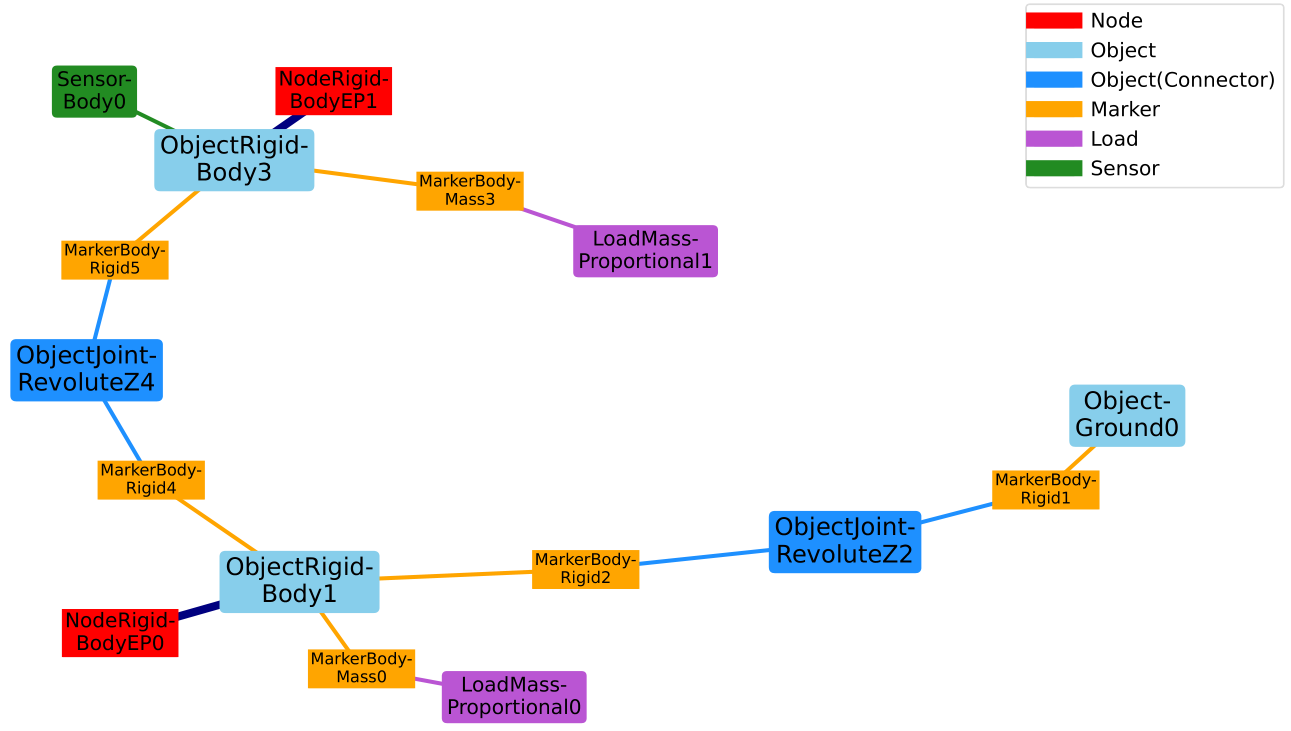
\includegraphics[width=0.9\textwidth]{figures/DrawSystemGraphExample}
  %\end{center}
  %\caption{System graph for rigid body tutorial (with option 3 for the first revolute joint). Numbers are always related to the node number, object number, etc.; note that colors are used to distinguish nodes, objects, markers, loads and sensors}
  %\label{fig_DrawSystemGraphExample}
%\end{figure}}
%\onlyRST{
%
%.. image:: docs/theDoc/figures/DrawSystemGraphExample.png
   %:width: 600
%
%}

\horizontalRuler\\
\noindent Before starting our simulation, we should adjust the solver parameters, especially the end time and the step size (no automatic step size for implicit solvers available!):
\pythonstyle\begin{lstlisting}
  simulationSettings = exu.SimulationSettings() #takes currently set values or default values

  tEnd = 4 #simulation time
  h = 1e-3 #step size
  simulationSettings.timeIntegration.numberOfSteps = int(tEnd/h)
  simulationSettings.timeIntegration.endTime = tEnd
  simulationSettings.timeIntegration.verboseMode = 1
  #simulationSettings.timeIntegration.simulateInRealtime = True
  simulationSettings.solutionSettings.solutionWritePeriod = 0.005 #store every 5 ms
\end{lstlisting}
The \texttt{verboseMode} tells the solver the amount of output during solving. Higher values (2, 3, ...) show residual vectors, jacobians, etc. for every time step, but slow down simulation significantly.
The option \texttt{simulateInRealtime} is used to view the model during simulation, while setting this false, 
the simulation finishes after fractions of a second. It should be set to false in general, 
while solution can be viewed using the \texttt{SolutionViewer()}.
With \texttt{solutionWritePeriod} you can adjust the frequency which is used to store the solution of the whole model, 
which may lead to very large files and may slow down simulation, but is used in the \texttt{SolutionViewer()} to reload the solution after simulation.

\noindent In order to improve visualization, there are hundreds of options, see Visualization settings in \refSection{sec:VisualizationSettingsMain}, some of them used here:
\pythonstyle\begin{lstlisting}
  SC.visualizationSettings.window.renderWindowSize = [1600,1200]
  SC.visualizationSettings.openGL.multiSampling = 4  #improved OpenGL rendering
  SC.visualizationSettings.general.autoFitScene = False

  SC.visualizationSettings.nodes.drawNodesAsPoint = False
  SC.visualizationSettings.nodes.showBasis = True #shows three RGB (=xyz) lines for node basis
\end{lstlisting}
The option \texttt{autoFitScene} is used in order to avoid zooming while loading the last saved render state, see below.

\noindent We can start the 3D visualization (Renderer) now:
\pythonstyle\begin{lstlisting}
  exu.StartRenderer()
\end{lstlisting}

\noindent In order to reload the model view of the last simulation (if there is any), we can use the following commands:
\pythonstyle\begin{lstlisting}
  if 'renderState' in exu.sys: #reload old view
      SC.SetRenderState(exu.sys['renderState'])

  mbs.WaitForUserToContinue() #stop before simulating
\end{lstlisting}
the function \texttt{WaitForUserToContinue()} waits with simulation until we press SPACE bar. This allows us to make some pre-checks.

\noindent Finally, the \mybold{index 2} (velocity level) implicit time integration (simulation) is started with:
\pythonstyle\begin{lstlisting}
  mbs.SolveDynamic(simulationSettings = simulationSettings,
                   solverType = exu.DynamicSolverType.TrapezoidalIndex2)
\end{lstlisting}
This solver is used in the present example, but should be considered with care as it leads to (small) drift of position constraints, linearly increasing in time. Using sufficiently small time steps, this effect is often negligible on the advantage of having a \mybold{energy-conserving integrator} (guaranteed for linear systems, but very often also for the nonlinear multibody system). Due to the velocity level, the integrator is less sensitive to consistent initial conditions on position level and compatible to frequent step size changes, however, initial jumps in velocities may never damp out in undamped systems.

\noindent Alternatively, an \mybold{index 3} implicit time integration -- the generalized-$\alpha$ method -- is started with the default settings for \texttt{solverType}:
\pythonstyle\begin{lstlisting}
  mbs.SolveDynamic(simulationSettings = simulationSettings)
\end{lstlisting}
Note that the \mybold{generalized-$\alpha$ method} includes numerical damping (adjusted with the spectral radius) for stabilization of index 3 constraints. This leads to effects every time the integrator is (re-)started, e.g., when adapting time step sizes. For fixed step sizes, this is \mybold{the recommended integrator}.

\noindent After simulation, the library would immediately exit (and jump back to iPython or close the terminal window). In order to avoid this, we can use \texttt{WaitForRenderEngineStopFlag()} to wait until we press key 'Q'.
\pythonstyle\begin{lstlisting}
  SC.WaitForRenderEngineStopFlag() #stop before closing
  exu.StopRenderer() #safely close rendering window!
\end{lstlisting}
If you entered everything correctly, the render window should show a nice animation of the 3D double pendulum after pressing the SPACE key. 
If we do not stop the renderer (\texttt{StopRenderer()}), it will stay open for further simulations. However, it is safer to always close the renderer at the end.

\noindent As the simulation will run very fast, if you did not set \texttt{simulateInRealtime} to true. However, you can reload the stored solution and view the stored steps interactively:
\pythonstyle\begin{lstlisting}
  mbs.SolutionViewer()
  #alternatively, we could load solution from a file:
  #sol = LoadSolutionFile('coordinatesSolution.txt')
  #mbs.SolutionViewer(sol)
\end{lstlisting}

\noindent Finally, we can plot our sensor, drawing the y-component of the sensor (check out the many options in \texttt{PlotSensor(...)} to conveniently represent results!):
\pythonstyle\begin{lstlisting}
  mbs.PlotSensor(sensorNumbers=[sens1],components=[1],closeAll=True)
\end{lstlisting}

\noindent \mybold{Congratulations}! You completed the rigid body tutorial, which gives you the ability to model multibody systems. Note that much more complicated models are possible, including feedback control or flexible bodies, see the Examples!


%+++++++++++++++++++++++++++++++++++++++++++++++++++++++++++++++++++++++++++++++
%+++++++++++++++++++++++++++++++++++++++++++++++++++++++++++++++++++++++++++++++
\mysubsection{Flexible beams tutorial}
This tutorial briefly introduces two simple planar beams and how to work with them with utility functions.
The python source code of the beam tutorial can be found at:
\bi
  \item[] \texttt{main/pythonDev/Examples/beamTutorial.py}
\ei
The tutorial uses the GeometricallyExactBeam2D, which is a shear deformable Reissner-Timoshenko beam, and a thin cable ANCFCable2D, which represents a large deformation Bernoulli-Euler beam.

\noindent The model includes two highly flexible planar with length 2m, height 0.005m, width 0.01m, 
Young's modulus 1e9N/m$^2$ and density 2000kg/m$^3$.
The shear deformable beam is rigidly attached to ground and the cable is rigidly attached to a moving ground.

\noindent We first import necessary libraries and set up a mbs. Note that utilities also include pi, sin, cos and sqrt.
\pythonstyle\begin{lstlisting}
  import exudyn as exu
  from exudyn.utilities import *
  import numpy as np

  SC = exu.SystemContainer()
  mbs = SC.AddSystem()
\end{lstlisting}

\noindent We define a set of beam parameters, discretization and geometry for both beam models.
\pythonstyle\begin{lstlisting}
  numberOfElements = 16
  L = 2                     # length of pendulum 
  E=2e11                    # steel
  rho=7800                  # elastomer
  h=0.005                   # height of rectangular beam element in m
  b=0.01                    # width of rectangular beam element in m
  A=b*h                     # cross sectional area of beam element in m^2
  I=b*h**3/12               # second moment of area of beam element in m^4
  nu = 0.3                  # Poisson's ratio
      
  EI = E*I
  EA = E*A
  rhoA = rho*A
  rhoI = rho*I
  ks = 10*(1+nu)/(12+11*nu) # shear correction factor
  G = E/(2*(1+nu))          # shear modulus
  GA = ks*G*A               # shear stiffness of beam

  g = [0,-9.81,0]           # gravity vector

  positionOfNode0 = [0,0,0] # 3D vector
  positionOfNode1 = [L,0,0] # 3D vector
\end{lstlisting}

\noindent Build geometrically exact 2D beam template (Timoshenko-Reissner), which includes all parameters
In order to create beams, we usually need to create 2D rigid body nodes, 
create beam elements, add constraints and loads.

\noindent However, there is a utility function \texttt{GenerateStraightBeam(...)}, 
which conveniently does this for straight beams, including discretization, constraints and gravity.
First, we create a beam template, which includes all beam parameters (this could also be another beam type):
\pythonstyle\begin{lstlisting}
  beamTemplate = Beam2D(nodeNumbers = [-1,-1], #added later
                        physicsMassPerLength=rhoA,
                        physicsCrossSectionInertia=rhoI,
                        physicsBendingStiffness=EI,
                        physicsAxialStiffness=EA,
                        physicsShearStiffness=GA,
                        physicsBendingDamping=0.02*EI,
                        visualization=VObjectBeamGeometricallyExact2D(drawHeight = h))
\end{lstlisting}

\noindent Now we use this template and call \texttt{GenerateStraightBeam}, which takes the nodal positions,
calculates according beam element lengths from discretization and could add constraints,
if \texttt{fixedConstraintsNode0} or \texttt{fixedConstraintsNode1} are not \texttt{None}.
\pythonstyle\begin{lstlisting}
  beamData = GenerateStraightBeam(mbs, positionOfNode0, positionOfNode1, 
                                  numberOfElements, beamTemplate, gravity= g, 
                                  fixedConstraintsNode0=[1,1,1], 
                                  fixedConstraintsNode1=None)
\end{lstlisting}

\noindent We perform the same operations for ANCF cable elemente (Bernoulli-Euler),
but in this case, we do not add constraints:
\pythonstyle\begin{lstlisting}
  beamTemplate = Cable2D(nodeNumbers = [-1,-1], #added later
                         physicsMassPerLength=rhoA,
                         physicsBendingStiffness=EI,
                         physicsAxialStiffness=EA,
                         physicsBendingDamping=0.02*EI,
                         visualization=VCable2D(drawHeight = h))

  cableData = GenerateStraightBeam(mbs, positionOfNode0, positionOfNode1, 
                                   numberOfElements, beamTemplate, gravity= g, 
                                   fixedConstraintsNode0=None, 
                                   fixedConstraintsNode1=None)
\end{lstlisting}

\noindent Now, we create a ground object and markers to attach cable with generic joint
\pythonstyle\begin{lstlisting}
  oGround = mbs.CreateGround(referencePosition=[0,0,0])
  mGround = mbs.AddMarker(MarkerBodyRigid(bodyNumber=oGround, localPosition=[0,0,0]))

  mCable = mbs.AddMarker(MarkerNodeRigid(nodeNumber=cableData[0][0]))
\end{lstlisting}

\noindent As we like to move the cable relative to ground, we employ a simple 
user function which prescribes relative rotation and (corotated) translation in the joint:
\pythonstyle\begin{lstlisting}
  def UFoffset(mbs, t, itemNumber, offsetUserFunctionParameters):
      x = SmoothStep(t, 2, 4, 0, 0.5)   #translate in local joint coordinates
      phi = SmoothStep(t, 5, 10, 0, pi) #rotates frame of mGround
      return [x, 0,0,0,0,phi]

\end{lstlisting}

\noindent Finally, we add the rigid joint (2D displacements and rotation around Z fixed) as GenericJoint.
Note that for 2D objects, we may only fix $X$- and $Y$-translations, as well as the $Z$-rotation
\pythonstyle\begin{lstlisting}
  mbs.AddObject(GenericJoint(markerNumbers=[mGround, mCable],
                             constrainedAxes=[1,1,0, 0,0,1],
                             offsetUserFunction=UFoffset,
                             visualization=VGenericJoint(axesRadius=0.01,
                                                         axesLength=0.02)))
\end{lstlisting}

\noindent As in the previous example, we just need to assemble and set up simulation parameters:
\pythonstyle\begin{lstlisting}
  mbs.Assemble()

  simulationSettings = exu.SimulationSettings()
      
  tEnd = 10
  stepSize = 0.005
  simulationSettings.timeIntegration.numberOfSteps = int(tEnd/stepSize)
  simulationSettings.timeIntegration.endTime = tEnd
  simulationSettings.timeIntegration.verboseMode = 1
  simulationSettings.solutionSettings.solutionWritePeriod = 0.005
  simulationSettings.solutionSettings.writeSolutionToFile = True

  simulationSettings.linearSolverType = exu.LinearSolverType.EigenSparse
  simulationSettings.timeIntegration.newton.useModifiedNewton = True #for faster simulation

  ## add some visualization settings
  SC.visualizationSettings.nodes.defaultSize = 0.01
  SC.visualizationSettings.nodes.drawNodesAsPoint = False #show beam nodes
  SC.visualizationSettings.bodies.beams.crossSectionFilled = True
\end{lstlisting}

\noindent Now start the solver with visualization and run the solution viewer afterwards,
because simulation may be faster than you can follow:
\pythonstyle\begin{lstlisting}
  exu.StartRenderer()
  mbs.SolveDynamic(simulationSettings)
  exu.StopRenderer()

  ## visualize computed solution:
  mbs.SolutionViewer()
\end{lstlisting}

\noindent The visualization window for the solution drawn at 6.5s is shown in \fig{fig_tutorial_beams}.
%
\LatexRSTfigure{figures/TutorialBeams}{fig_tutorial_beams}{15cm}{500}{Render window showing the deformed state of the two beams at 6.5s. The lower beam is fixed at the left end, while the upper beam's support is translated and rotated.}
%

\noindent This example should give you a good starting point to create beam models.
See further examples, and more advanced functions, e.g., to create curved beam or reeving systems.
There are also a sliding joint as well as axially moving beams and contact between beams and sheaves.

\noindent 3D beams are still under development and include less functionality. In case, send a request at the GitHub discussion or issues.

